\documentclass[1p]{elsarticle_modified}
%\bibliographystyle{elsarticle-num}

%\usepackage[colorlinks]{hyperref}
%\usepackage{abbrmath_seonhwa} %\Abb, \Ascr, \Acal ,\Abf, \Afrak
\usepackage{amsfonts}
\usepackage{amssymb}
\usepackage{amsmath}
\usepackage{amsthm}
\usepackage{scalefnt}
\usepackage{amsbsy}
\usepackage{kotex}
\usepackage{caption}
\usepackage{subfig}
\usepackage{color}
\usepackage{graphicx}
\usepackage{xcolor} %% white, black, red, green, blue, cyan, magenta, yellow
\usepackage{float}
\usepackage{setspace}
\usepackage{hyperref}

\usepackage{tikz}
\usetikzlibrary{arrows}

\usepackage{multirow}
\usepackage{array} % fixed length table
\usepackage{hhline}

%%%%%%%%%%%%%%%%%%%%%
\makeatletter
\renewcommand*\env@matrix[1][\arraystretch]{%
	\edef\arraystretch{#1}%
	\hskip -\arraycolsep
	\let\@ifnextchar\new@ifnextchar
	\array{*\c@MaxMatrixCols c}}
\makeatother %https://tex.stackexchange.com/questions/14071/how-can-i-increase-the-line-spacing-in-a-matrix
%%%%%%%%%%%%%%%

\usepackage[normalem]{ulem}

\newcommand{\msout}[1]{\ifmmode\text{\sout{\ensuremath{#1}}}\else\sout{#1}\fi}
%SOURCE: \msout is \stkout macro in https://tex.stackexchange.com/questions/20609/strikeout-in-math-mode

\newcommand{\cancel}[1]{
	\ifmmode
	{\color{red}\msout{#1}}
	\else
	{\color{red}\sout{#1}}
	\fi
}

\newcommand{\add}[1]{
	{\color{blue}\uwave{#1}}
}

\newcommand{\replace}[2]{
	\ifmmode
	{\color{red}\msout{#1}}{\color{blue}\uwave{#2}}
	\else
	{\color{red}\sout{#1}}{\color{blue}\uwave{#2}}
	\fi
}

\newcommand{\Sol}{\mathcal{S}} %segment
\newcommand{\D}{D} %diagram
\newcommand{\A}{\mathcal{A}} %arc


%%%%%%%%%%%%%%%%%%%%%%%%%%%%%5 test

\def\sl{\operatorname{\textup{SL}}(2,\Cbb)}
\def\psl{\operatorname{\textup{PSL}}(2,\Cbb)}
\def\quan{\mkern 1mu \triangleright \mkern 1mu}

\theoremstyle{definition}
\newtheorem{thm}{Theorem}[section]
\newtheorem{prop}[thm]{Proposition}
\newtheorem{lem}[thm]{Lemma}
\newtheorem{ques}[thm]{Question}
\newtheorem{cor}[thm]{Corollary}
\newtheorem{defn}[thm]{Definition}
\newtheorem{exam}[thm]{Example}
\newtheorem{rmk}[thm]{Remark}
\newtheorem{alg}[thm]{Algorithm}

\newcommand{\I}{\sqrt{-1}}
\begin{document}

%\begin{frontmatter}
%
%\title{Boundary parabolic representations of knots up to 8 crossings}
%
%%% Group authors per affiliation:
%\author{Yunhi Cho} 
%\address{Department of Mathematics, University of Seoul, Seoul, Korea}
%\ead{yhcho@uos.ac.kr}
%
%
%\author{Seonhwa Kim} %\fnref{s_kim}}
%\address{Center for Geometry and Physics, Institute for Basic Science, Pohang, 37673, Korea}
%\ead{ryeona17@ibs.re.kr}
%
%\author{Hyuk Kim}
%\address{Department of Mathematical Sciences, Seoul National University, Seoul 08826, Korea}
%\ead{hyukkim@snu.ac.kr}
%
%\author{Seokbeom Yoon}
%\address{Department of Mathematical Sciences, Seoul National University, Seoul, 08826,  Korea}
%\ead{sbyoon15@snu.ac.kr}
%
%\begin{abstract}
%We find all boundary parabolic representation of knots up to 8 crossings.
%
%\end{abstract}
%\begin{keyword}
%    \MSC[2010] 57M25 
%\end{keyword}
%
%\end{frontmatter}

%\linenumbers
%\tableofcontents
%
\newcommand\colored[1]{\textcolor{white}{\rule[-0.35ex]{0.8em}{1.4ex}}\kern-0.8em\color{red} #1}%
%\newcommand\colored[1]{\textcolor{white}{ #1}\kern-2.17ex	\textcolor{white}{ #1}\kern-1.81ex	\textcolor{white}{ #1}\kern-2.15ex\color{red}#1	}

{\Large $\underline{12n_{0579}~(K12n_{0579})}$}

\setlength{\tabcolsep}{10pt}
\renewcommand{\arraystretch}{1.6}
\vspace{1cm}\begin{tabular}{m{100pt}>{\centering\arraybackslash}m{274pt}}
\multirow{5}{120pt}{
	\centering
	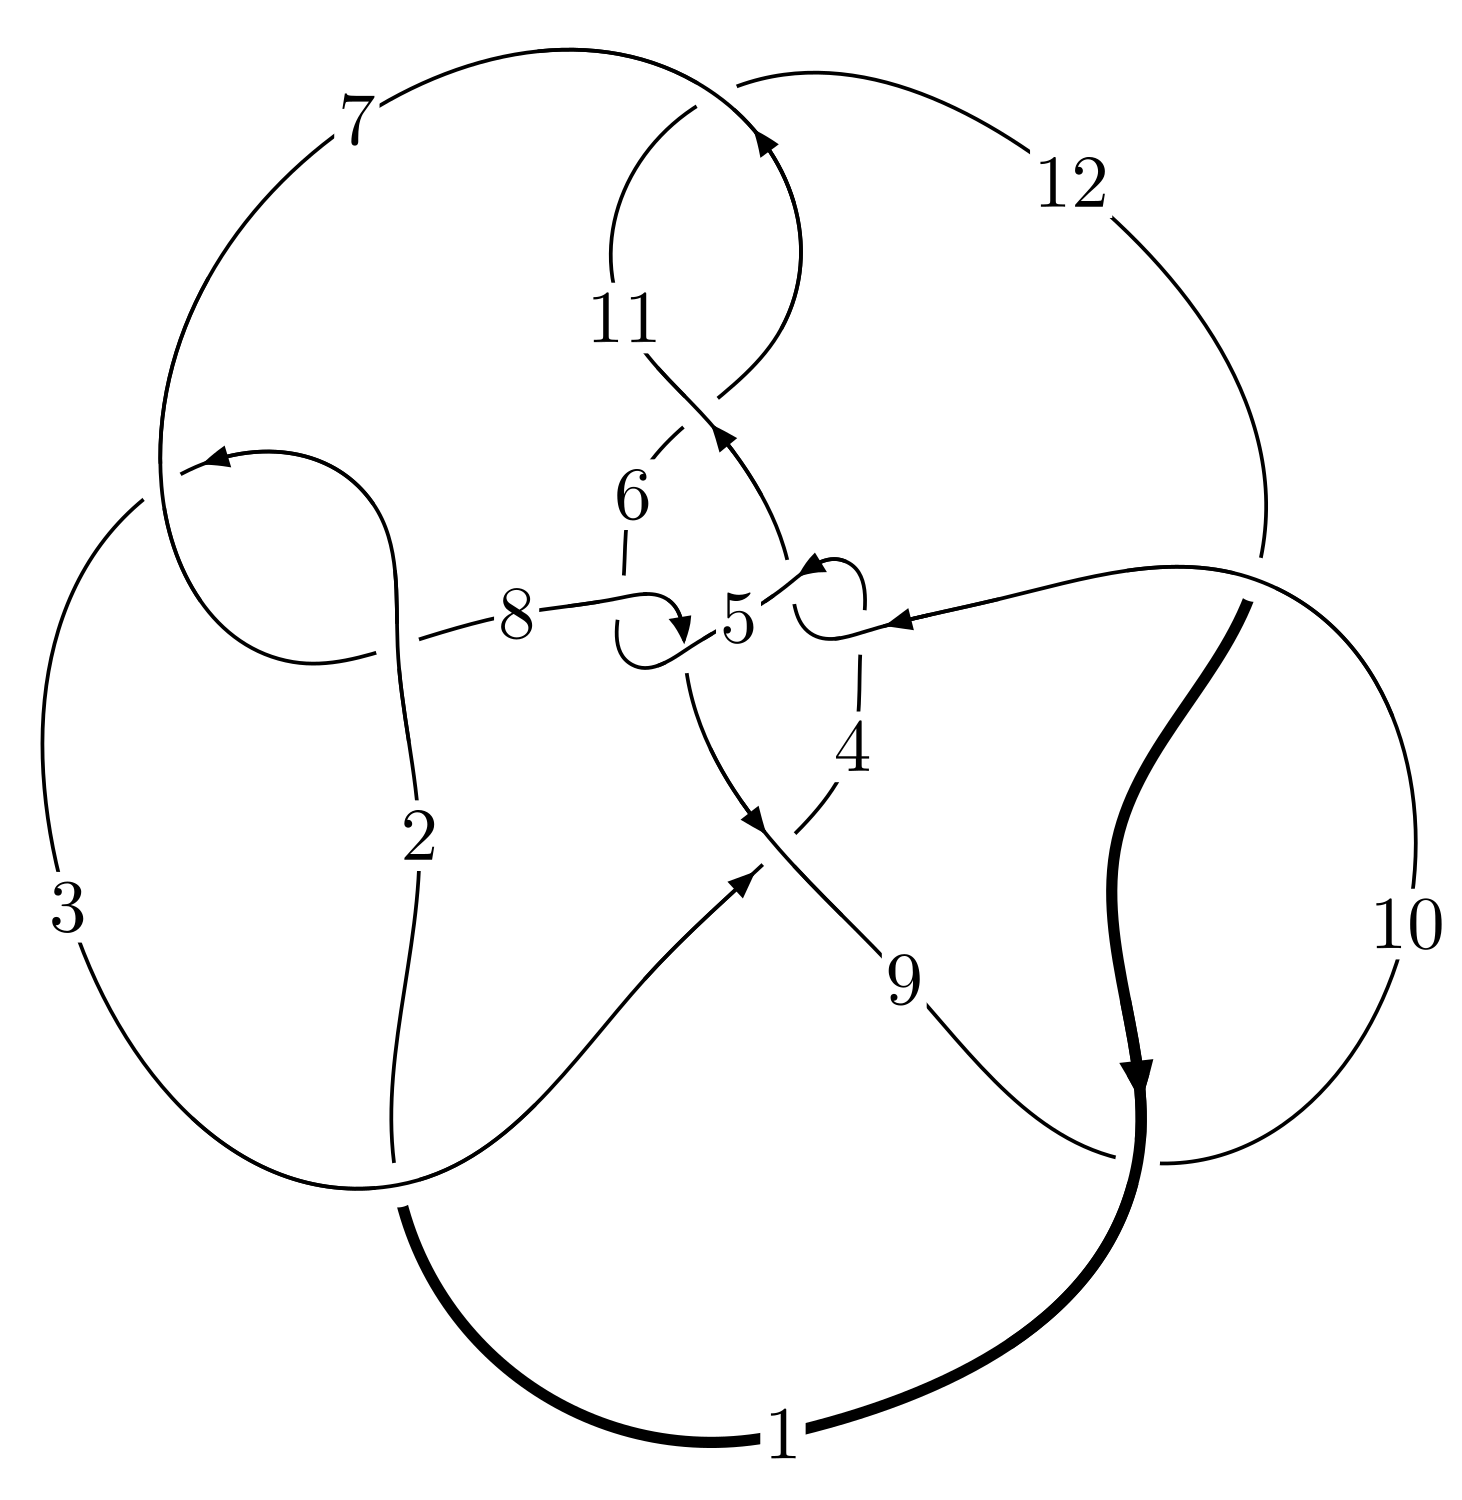
\includegraphics[width=112pt]{../../../GIT/diagram.site/Diagrams/png/2668_12n_0579.png}\\
\ \ \ A knot diagram\footnotemark}&
\allowdisplaybreaks
\textbf{Linearized knot diagam} \\
\cline{2-2}
 &
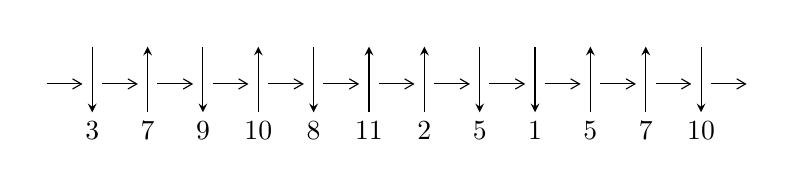
\begin{tikzpicture}[x=20pt, y=17pt]
	% nodes
	\node (C0) at (0, 0) {};
	\node (C1) at (1, 0) {};
	\node (C1U) at (1, +1) {};
	\node (C1D) at (1, -1) {3};

	\node (C2) at (2, 0) {};
	\node (C2U) at (2, +1) {};
	\node (C2D) at (2, -1) {7};

	\node (C3) at (3, 0) {};
	\node (C3U) at (3, +1) {};
	\node (C3D) at (3, -1) {9};

	\node (C4) at (4, 0) {};
	\node (C4U) at (4, +1) {};
	\node (C4D) at (4, -1) {10};

	\node (C5) at (5, 0) {};
	\node (C5U) at (5, +1) {};
	\node (C5D) at (5, -1) {8};

	\node (C6) at (6, 0) {};
	\node (C6U) at (6, +1) {};
	\node (C6D) at (6, -1) {11};

	\node (C7) at (7, 0) {};
	\node (C7U) at (7, +1) {};
	\node (C7D) at (7, -1) {2};

	\node (C8) at (8, 0) {};
	\node (C8U) at (8, +1) {};
	\node (C8D) at (8, -1) {5};

	\node (C9) at (9, 0) {};
	\node (C9U) at (9, +1) {};
	\node (C9D) at (9, -1) {1};

	\node (C10) at (10, 0) {};
	\node (C10U) at (10, +1) {};
	\node (C10D) at (10, -1) {5};

	\node (C11) at (11, 0) {};
	\node (C11U) at (11, +1) {};
	\node (C11D) at (11, -1) {7};

	\node (C12) at (12, 0) {};
	\node (C12U) at (12, +1) {};
	\node (C12D) at (12, -1) {10};
	\node (C13) at (13, 0) {};

	% arrows
	\draw[->,>={angle 60}]
	(C0) edge (C1) (C1) edge (C2) (C2) edge (C3) (C3) edge (C4) (C4) edge (C5) (C5) edge (C6) (C6) edge (C7) (C7) edge (C8) (C8) edge (C9) (C9) edge (C10) (C10) edge (C11) (C11) edge (C12) (C12) edge (C13) ;	\draw[->,>=stealth]
	(C1U) edge (C1D) (C2D) edge (C2U) (C3U) edge (C3D) (C4D) edge (C4U) (C5U) edge (C5D) (C6D) edge (C6U) (C7D) edge (C7U) (C8U) edge (C8D) (C9U) edge (C9D) (C10D) edge (C10U) (C11D) edge (C11U) (C12U) edge (C12D) ;
	\end{tikzpicture} \\
\hhline{~~} \\& 
\textbf{Solving Sequence} \\ \cline{2-2} 
 &
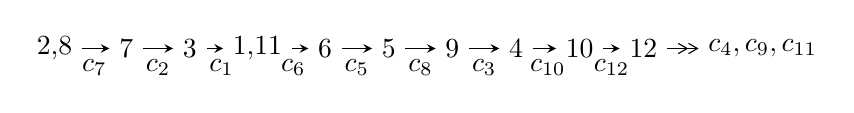
\begin{tikzpicture}[x=23pt, y=7pt]
	% node
	\node (A0) at (-1/8, 0) {2,8};
	\node (A1) at (1, 0) {7};
	\node (A2) at (2, 0) {3};
	\node (A3) at (49/16, 0) {1,11};
	\node (A4) at (33/8, 0) {6};
	\node (A5) at (41/8, 0) {5};
	\node (A6) at (49/8, 0) {9};
	\node (A7) at (57/8, 0) {4};
	\node (A8) at (65/8, 0) {10};
	\node (A9) at (73/8, 0) {12};
	\node (C1) at (1/2, -1) {$c_{7}$};
	\node (C2) at (3/2, -1) {$c_{2}$};
	\node (C3) at (5/2, -1) {$c_{1}$};
	\node (C4) at (29/8, -1) {$c_{6}$};
	\node (C5) at (37/8, -1) {$c_{5}$};
	\node (C6) at (45/8, -1) {$c_{8}$};
	\node (C7) at (53/8, -1) {$c_{3}$};
	\node (C8) at (61/8, -1) {$c_{10}$};
	\node (C9) at (69/8, -1) {$c_{12}$};
	\node (A10) at (11, 0) {$c_{4},c_{9},c_{11}$};

	% edge
	\draw[->,>=stealth]	
	(A0) edge (A1) (A1) edge (A2) (A2) edge (A3) (A3) edge (A4) (A4) edge (A5) (A5) edge (A6) (A6) edge (A7) (A7) edge (A8) (A8) edge (A9) ;
	\draw[->>,>={angle 60}]	
	(A9) edge (A10);
\end{tikzpicture} \\ 

\end{tabular} \\

\footnotetext{
The image of knot diagram is generated by the software ``\textbf{Draw programme}" developed by Andrew Bartholomew(\url{http://www.layer8.co.uk/maths/draw/index.htm\#Running-draw}), where we modified some parts for our purpose(\url{https://github.com/CATsTAILs/LinksPainter}).
}\phantom \\ \newline 
\centering \textbf{Ideals for irreducible components\footnotemark of $X_{\text{par}}$} 
 
\begin{align*}
I^u_{1}&=\langle 
-11 u^{19}+125 u^{18}+\cdots+8 b+264,\;-11 u^{19}+91 u^{18}+\cdots+16 a-128,\;u^{20}-11 u^{19}+\cdots-80 u+16\rangle \\
I^u_{2}&=\langle 
u^{15}+2 u^{14}+\cdots+b+1,\;-2 u^{15}-2 u^{14}+\cdots+a+4,\\
\phantom{I^u_{2}}&\phantom{= \langle  }u^{16}+u^{15}+4 u^{14}+3 u^{13}+10 u^{12}+5 u^{11}+15 u^{10}+4 u^9+17 u^8+u^7+14 u^6-2 u^5+10 u^4-2 u^3+4 u^2- u+1\rangle \\
\\
\end{align*}
\raggedright * 2 irreducible components of $\dim_{\mathbb{C}}=0$, with total 36 representations.\\
\footnotetext{All coefficients of polynomials are rational numbers. But the coefficients are sometimes approximated in decimal forms when there is not enough margin.}
\newpage
\renewcommand{\arraystretch}{1}
\centering \section*{I. $I^u_{1}= \langle -11 u^{19}+125 u^{18}+\cdots+8 b+264,\;-11 u^{19}+91 u^{18}+\cdots+16 a-128,\;u^{20}-11 u^{19}+\cdots-80 u+16 \rangle$}
\flushleft \textbf{(i) Arc colorings}\\
\begin{tabular}{m{7pt} m{180pt} m{7pt} m{180pt} }
\flushright $a_{2}=$&$\begin{pmatrix}0\\u\end{pmatrix}$ \\
\flushright $a_{8}=$&$\begin{pmatrix}1\\0\end{pmatrix}$ \\
\flushright $a_{7}=$&$\begin{pmatrix}1\\u^2\end{pmatrix}$ \\
\flushright $a_{3}=$&$\begin{pmatrix}u\\u^3+u\end{pmatrix}$ \\
\flushright $a_{1}=$&$\begin{pmatrix}u^3\\u^5+u^3+u\end{pmatrix}$ \\
\flushright $a_{11}=$&$\begin{pmatrix}\frac{11}{16} u^{19}-\frac{91}{16} u^{18}+\cdots-23 u+8\\\frac{11}{8} u^{19}-\frac{125}{8} u^{18}+\cdots+140 u-33\end{pmatrix}$ \\
\flushright $a_{6}=$&$\begin{pmatrix}-\frac{1}{4} u^{19}+\frac{5}{2} u^{18}+\cdots-10 u+\frac{5}{2}\\\frac{1}{4} u^{19}-\frac{9}{4} u^{18}+\cdots-\frac{15}{2} u^2+\frac{3}{2} u\end{pmatrix}$ \\
\flushright $a_{5}=$&$\begin{pmatrix}\frac{1}{4} u^{18}-\frac{9}{4} u^{17}+\cdots-\frac{17}{2} u+\frac{5}{2}\\\frac{1}{4} u^{19}-\frac{9}{4} u^{18}+\cdots-\frac{15}{2} u^2+\frac{3}{2} u\end{pmatrix}$ \\
\flushright $a_{9}=$&$\begin{pmatrix}2 u^{19}-\frac{83}{4} u^{18}+\cdots+\frac{419}{4} u-21\\\frac{5}{4} u^{19}-\frac{29}{2} u^{18}+\cdots+122 u-28\end{pmatrix}$ \\
\flushright $a_{4}=$&$\begin{pmatrix}-\frac{59}{16} u^{19}+\frac{475}{16} u^{18}+\cdots+147 u-48\\-\frac{79}{8} u^{19}+\frac{769}{8} u^{18}+\cdots-274 u+45\end{pmatrix}$ \\
\flushright $a_{10}=$&$\begin{pmatrix}7 u^{19}-\frac{291}{4} u^{18}+\cdots+\frac{1491}{4} u-77\\4 u^{19}-\frac{193}{4} u^{18}+\cdots+478 u-112\end{pmatrix}$ \\
\flushright $a_{12}=$&$\begin{pmatrix}\frac{1}{16} u^{19}+\frac{3}{16} u^{18}+\cdots-22 u+5\\\frac{7}{8} u^{19}-\frac{73}{8} u^{18}+\cdots+70 u-17\end{pmatrix}$\\&\end{tabular}
\flushleft \textbf{(ii) Obstruction class $= -1$}\\~\\
\flushleft \textbf{(iii) Cusp Shapes $= \frac{19}{2} u^{19}-\frac{231}{2} u^{18}+698 u^{17}-\frac{5601}{2} u^{16}+8288 u^{15}-\frac{38259}{2} u^{14}+\frac{71281}{2} u^{13}-54910 u^{12}+\frac{142795}{2} u^{11}-\frac{159597}{2} u^{10}+77978 u^9-67433 u^8+51758 u^7-35082 u^6+20913 u^5-\frac{22571}{2} u^4+\frac{11687}{2} u^3-2983 u^2+1252 u-290$}\\~\\
\newpage\renewcommand{\arraystretch}{1}
\flushleft \textbf{(iv) u-Polynomials at the component}\newline \\
\begin{tabular}{m{50pt}|m{274pt}}
Crossings & \hspace{64pt}u-Polynomials at each crossing \\
\hline $$\begin{aligned}c_{1}\end{aligned}$$&$\begin{aligned}
&u^{20}+7 u^{19}+\cdots+640 u+256
\end{aligned}$\\
\hline $$\begin{aligned}c_{2},c_{7}\end{aligned}$$&$\begin{aligned}
&u^{20}+11 u^{19}+\cdots+80 u+16
\end{aligned}$\\
\hline $$\begin{aligned}c_{3}\end{aligned}$$&$\begin{aligned}
&u^{20}+2 u^{19}+\cdots+55 u+1477
\end{aligned}$\\
\hline $$\begin{aligned}c_{4},c_{10}\end{aligned}$$&$\begin{aligned}
&u^{20}+21 u^{18}+\cdots+59 u+42
\end{aligned}$\\
\hline $$\begin{aligned}c_{5},c_{8}\end{aligned}$$&$\begin{aligned}
&u^{20}-3 u^{19}+\cdots-2 u+1
\end{aligned}$\\
\hline $$\begin{aligned}c_{6},c_{11}\end{aligned}$$&$\begin{aligned}
&u^{20}+u^{19}+\cdots+u+1
\end{aligned}$\\
\hline $$\begin{aligned}c_{9},c_{12}\end{aligned}$$&$\begin{aligned}
&u^{20}-3 u^{19}+\cdots-4 u+1
\end{aligned}$\\
\hline
\end{tabular}\\~\\
\newpage\renewcommand{\arraystretch}{1}
\flushleft \textbf{(v) Riley Polynomials at the component}\newline \\
\begin{tabular}{m{50pt}|m{274pt}}
Crossings & \hspace{64pt}Riley Polynomials at each crossing \\
\hline $$\begin{aligned}c_{1}\end{aligned}$$&$\begin{aligned}
&y^{20}+11 y^{19}+\cdots+1155072 y+65536
\end{aligned}$\\
\hline $$\begin{aligned}c_{2},c_{7}\end{aligned}$$&$\begin{aligned}
&y^{20}+7 y^{19}+\cdots+640 y+256
\end{aligned}$\\
\hline $$\begin{aligned}c_{3}\end{aligned}$$&$\begin{aligned}
&y^{20}-22 y^{19}+\cdots-6941971 y+2181529
\end{aligned}$\\
\hline $$\begin{aligned}c_{4},c_{10}\end{aligned}$$&$\begin{aligned}
&y^{20}+42 y^{19}+\cdots+22475 y+1764
\end{aligned}$\\
\hline $$\begin{aligned}c_{5},c_{8}\end{aligned}$$&$\begin{aligned}
&y^{20}-43 y^{19}+\cdots+54 y+1
\end{aligned}$\\
\hline $$\begin{aligned}c_{6},c_{11}\end{aligned}$$&$\begin{aligned}
&y^{20}+35 y^{19}+\cdots-7 y+1
\end{aligned}$\\
\hline $$\begin{aligned}c_{9},c_{12}\end{aligned}$$&$\begin{aligned}
&y^{20}+3 y^{19}+\cdots+10 y+1
\end{aligned}$\\
\hline
\end{tabular}\\~\\
\newpage\flushleft \textbf{(vi) Complex Volumes and Cusp Shapes}
$$\begin{array}{c|c|c}  
\text{Solutions to }I^u_{1}& \I (\text{vol} + \sqrt{-1}CS) & \text{Cusp shape}\\
 \hline 
\begin{aligned}
u &= -0.374976 + 0.845868 I \\
a &= \phantom{-}0.304346 - 0.429032 I \\
b &= -0.004516 + 0.301455 I\end{aligned}
 & -0.45102 - 2.09204 I & \phantom{-}1.92279 + 3.74231 I \\ \hline\begin{aligned}
u &= -0.374976 - 0.845868 I \\
a &= \phantom{-}0.304346 + 0.429032 I \\
b &= -0.004516 - 0.301455 I\end{aligned}
 & -0.45102 + 2.09204 I & \phantom{-}1.92279 - 3.74231 I \\ \hline\begin{aligned}
u &= \phantom{-}0.282023 + 1.083820 I \\
a &= \phantom{-}0.39008 - 1.59752 I \\
b &= \phantom{-}0.80004 + 1.16903 I\end{aligned}
 & -3.81050 + 0.28255 I & -5.79309 - 4.21842 I \\ \hline\begin{aligned}
u &= \phantom{-}0.282023 - 1.083820 I \\
a &= \phantom{-}0.39008 + 1.59752 I \\
b &= \phantom{-}0.80004 - 1.16903 I\end{aligned}
 & -3.81050 - 0.28255 I & -5.79309 + 4.21842 I \\ \hline\begin{aligned}
u &= \phantom{-}0.684540 + 0.363080 I \\
a &= \phantom{-}0.592020 + 0.442074 I \\
b &= -0.478548 + 1.089890 I\end{aligned}
 & \phantom{-}0.21798 - 2.21625 I & \phantom{-}4.78739 + 3.65383 I \\ \hline\begin{aligned}
u &= \phantom{-}0.684540 - 0.363080 I \\
a &= \phantom{-}0.592020 - 0.442074 I \\
b &= -0.478548 - 1.089890 I\end{aligned}
 & \phantom{-}0.21798 + 2.21625 I & \phantom{-}4.78739 - 3.65383 I \\ \hline\begin{aligned}
u &= \phantom{-}0.854003 + 0.892169 I \\
a &= \phantom{-}0.506066 + 0.028446 I \\
b &= -0.446717 + 0.529073 I\end{aligned}
 & \phantom{-}7.04464 + 1.66022 I & \phantom{-}3.68035 + 3.33714 I \\ \hline\begin{aligned}
u &= \phantom{-}0.854003 - 0.892169 I \\
a &= \phantom{-}0.506066 - 0.028446 I \\
b &= -0.446717 - 0.529073 I\end{aligned}
 & \phantom{-}7.04464 - 1.66022 I & \phantom{-}3.68035 - 3.33714 I \\ \hline\begin{aligned}
u &= \phantom{-}0.557284 + 1.103710 I \\
a &= -0.91469 + 1.63155 I \\
b &= -0.64503 - 1.83466 I\end{aligned}
 & -1.93145 + 7.03308 I & \phantom{-}4.92278 - 7.07574 I \\ \hline\begin{aligned}
u &= \phantom{-}0.557284 - 1.103710 I \\
a &= -0.91469 - 1.63155 I \\
b &= -0.64503 + 1.83466 I\end{aligned}
 & -1.93145 - 7.03308 I & \phantom{-}4.92278 + 7.07574 I\\
 \hline 
 \end{array}$$\newpage$$\begin{array}{c|c|c}  
\text{Solutions to }I^u_{1}& \I (\text{vol} + \sqrt{-1}CS) & \text{Cusp shape}\\
 \hline 
\begin{aligned}
u &= \phantom{-}0.843906 + 0.926863 I \\
a &= -0.147807 + 0.491044 I \\
b &= -0.393488 - 0.559354 I\end{aligned}
 & \phantom{-}6.93872 + 4.64909 I & \phantom{-}6.55707 - 9.56183 I \\ \hline\begin{aligned}
u &= \phantom{-}0.843906 - 0.926863 I \\
a &= -0.147807 - 0.491044 I \\
b &= -0.393488 + 0.559354 I\end{aligned}
 & \phantom{-}6.93872 - 4.64909 I & \phantom{-}6.55707 + 9.56183 I \\ \hline\begin{aligned}
u &= -0.408387 + 0.451294 I \\
a &= \phantom{-}0.739810 + 0.208470 I \\
b &= -0.306448 + 0.078414 I\end{aligned}
 & \phantom{-}0.672383 - 0.998162 I & \phantom{-}5.05990 + 5.48797 I \\ \hline\begin{aligned}
u &= -0.408387 - 0.451294 I \\
a &= \phantom{-}0.739810 - 0.208470 I \\
b &= -0.306448 - 0.078414 I\end{aligned}
 & \phantom{-}0.672383 + 0.998162 I & \phantom{-}5.05990 - 5.48797 I \\ \hline\begin{aligned}
u &= \phantom{-}1.50042 + 0.03858 I \\
a &= \phantom{-}0.039797 - 0.614362 I \\
b &= -0.02477 + 1.84088 I\end{aligned}
 & -10.85850 - 3.49800 I & \phantom{-}1.91176 + 2.12217 I \\ \hline\begin{aligned}
u &= \phantom{-}1.50042 - 0.03858 I \\
a &= \phantom{-}0.039797 + 0.614362 I \\
b &= -0.02477 - 1.84088 I\end{aligned}
 & -10.85850 + 3.49800 I & \phantom{-}1.91176 - 2.12217 I \\ \hline\begin{aligned}
u &= \phantom{-}0.75634 + 1.50493 I \\
a &= \phantom{-}0.88084 - 1.46544 I \\
b &= \phantom{-}0.16039 + 1.88216 I\end{aligned}
 & -15.5277 + 4.3237 I & \phantom{-0.000000 }      -6
0. 10   - 0.824539 I \\ \hline\begin{aligned}
u &= \phantom{-}0.75634 - 1.50493 I \\
a &= \phantom{-}0.88084 + 1.46544 I \\
b &= \phantom{-}0.16039 - 1.88216 I\end{aligned}
 & -15.5277 - 4.3237 I & \phantom{-0.000000 -}     -6
0. 10   + 0.824539 I \\ \hline\begin{aligned}
u &= \phantom{-}0.80485 + 1.48779 I \\
a &= -0.89046 + 1.47434 I \\
b &= -0.16092 - 1.93495 I\end{aligned}
 & -15.1932 + 11.4769 I & \phantom{-0.000000 } 0. - 4.87637 I \\ \hline\begin{aligned}
u &= \phantom{-}0.80485 - 1.48779 I \\
a &= -0.89046 - 1.47434 I \\
b &= -0.16092 + 1.93495 I\end{aligned}
 & -15.1932 - 11.4769 I & \phantom{-0.000000 -}0. + 4.87637 I\\
 \hline 
 \end{array}$$\newpage\newpage\renewcommand{\arraystretch}{1}
\centering \section*{II. $I^u_{2}= \langle u^{15}+2 u^{14}+\cdots+b+1,\;-2 u^{15}-2 u^{14}+\cdots+a+4,\;u^{16}+u^{15}+\cdots- u+1 \rangle$}
\flushleft \textbf{(i) Arc colorings}\\
\begin{tabular}{m{7pt} m{180pt} m{7pt} m{180pt} }
\flushright $a_{2}=$&$\begin{pmatrix}0\\u\end{pmatrix}$ \\
\flushright $a_{8}=$&$\begin{pmatrix}1\\0\end{pmatrix}$ \\
\flushright $a_{7}=$&$\begin{pmatrix}1\\u^2\end{pmatrix}$ \\
\flushright $a_{3}=$&$\begin{pmatrix}u\\u^3+u\end{pmatrix}$ \\
\flushright $a_{1}=$&$\begin{pmatrix}u^3\\u^5+u^3+u\end{pmatrix}$ \\
\flushright $a_{11}=$&$\begin{pmatrix}2 u^{15}+2 u^{14}+\cdots+5 u-4\\- u^{15}-2 u^{14}+\cdots-4 u-1\end{pmatrix}$ \\
\flushright $a_{6}=$&$\begin{pmatrix}u^{14}+u^{13}+\cdots-2 u+4\\u^{15}+u^{14}+\cdots+3 u-1\end{pmatrix}$ \\
\flushright $a_{5}=$&$\begin{pmatrix}u^{15}+2 u^{14}+\cdots+u+3\\u^{15}+u^{14}+\cdots+3 u-1\end{pmatrix}$ \\
\flushright $a_{9}=$&$\begin{pmatrix}2 u^{15}+u^{14}+\cdots+u-2\\- u^{15}-2 u^{14}+\cdots-2 u-1\end{pmatrix}$ \\
\flushright $a_{4}=$&$\begin{pmatrix}- u^{15}+u^{14}+\cdots-7 u+5\\u^{12}+u^{11}+\cdots+2 u+1\end{pmatrix}$ \\
\flushright $a_{10}=$&$\begin{pmatrix}2 u^{15}+u^{14}+\cdots+2 u-2\\-2 u^{15}-3 u^{14}+\cdots-2 u^2-3 u\end{pmatrix}$ \\
\flushright $a_{12}=$&$\begin{pmatrix}u^{15}+u^{14}+\cdots+3 u-5\\- u^{15}-3 u^{14}+\cdots-3 u-1\end{pmatrix}$\\&\end{tabular}
\flushleft \textbf{(ii) Obstruction class $= 1$}\\~\\
\flushleft \textbf{(iii) Cusp Shapes $= -3 u^{14}-7 u^{13}-13 u^{12}-19 u^{11}-31 u^{10}-41 u^9-44 u^8-45 u^7-43 u^6-39 u^5-25 u^4-13 u^3-10 u^2-9 u-2$}\\~\\
\newpage\renewcommand{\arraystretch}{1}
\flushleft \textbf{(iv) u-Polynomials at the component}\newline \\
\begin{tabular}{m{50pt}|m{274pt}}
Crossings & \hspace{64pt}u-Polynomials at each crossing \\
\hline $$\begin{aligned}c_{1}\end{aligned}$$&$\begin{aligned}
&u^{16}-7 u^{15}+\cdots-7 u+1
\end{aligned}$\\
\hline $$\begin{aligned}c_{2}\end{aligned}$$&$\begin{aligned}
&u^{16}- u^{15}+\cdots+u+1
\end{aligned}$\\
\hline $$\begin{aligned}c_{3}\end{aligned}$$&$\begin{aligned}
&u^{16}- u^{15}+\cdots-15 u+5
\end{aligned}$\\
\hline $$\begin{aligned}c_{4}\end{aligned}$$&$\begin{aligned}
&u^{16}- u^{15}+\cdots+9 u^2+5
\end{aligned}$\\
\hline $$\begin{aligned}c_{5}\end{aligned}$$&$\begin{aligned}
&u^{16}-2 u^{15}+\cdots-2 u^2+1
\end{aligned}$\\
\hline $$\begin{aligned}c_{6}\end{aligned}$$&$\begin{aligned}
&u^{16}-3 u^{14}+\cdots+u+1
\end{aligned}$\\
\hline $$\begin{aligned}c_{7}\end{aligned}$$&$\begin{aligned}
&u^{16}+u^{15}+\cdots- u+1
\end{aligned}$\\
\hline $$\begin{aligned}c_{8}\end{aligned}$$&$\begin{aligned}
&u^{16}+2 u^{15}+\cdots-2 u^2+1
\end{aligned}$\\
\hline $$\begin{aligned}c_{9}\end{aligned}$$&$\begin{aligned}
&u^{16}-6 u^{15}+\cdots-4 u+1
\end{aligned}$\\
\hline $$\begin{aligned}c_{10}\end{aligned}$$&$\begin{aligned}
&u^{16}+u^{15}+\cdots+9 u^2+5
\end{aligned}$\\
\hline $$\begin{aligned}c_{11}\end{aligned}$$&$\begin{aligned}
&u^{16}-3 u^{14}+\cdots- u+1
\end{aligned}$\\
\hline $$\begin{aligned}c_{12}\end{aligned}$$&$\begin{aligned}
&u^{16}+6 u^{15}+\cdots+4 u+1
\end{aligned}$\\
\hline
\end{tabular}\\~\\
\newpage\renewcommand{\arraystretch}{1}
\flushleft \textbf{(v) Riley Polynomials at the component}\newline \\
\begin{tabular}{m{50pt}|m{274pt}}
Crossings & \hspace{64pt}Riley Polynomials at each crossing \\
\hline $$\begin{aligned}c_{1}\end{aligned}$$&$\begin{aligned}
&y^{16}+11 y^{15}+\cdots+15 y+1
\end{aligned}$\\
\hline $$\begin{aligned}c_{2},c_{7}\end{aligned}$$&$\begin{aligned}
&y^{16}+7 y^{15}+\cdots+7 y+1
\end{aligned}$\\
\hline $$\begin{aligned}c_{3}\end{aligned}$$&$\begin{aligned}
&y^{16}+13 y^{15}+\cdots+415 y+25
\end{aligned}$\\
\hline $$\begin{aligned}c_{4},c_{10}\end{aligned}$$&$\begin{aligned}
&y^{16}-3 y^{15}+\cdots+90 y+25
\end{aligned}$\\
\hline $$\begin{aligned}c_{5},c_{8}\end{aligned}$$&$\begin{aligned}
&y^{16}+4 y^{15}+\cdots-4 y+1
\end{aligned}$\\
\hline $$\begin{aligned}c_{6},c_{11}\end{aligned}$$&$\begin{aligned}
&y^{16}-6 y^{15}+\cdots+7 y+1
\end{aligned}$\\
\hline $$\begin{aligned}c_{9},c_{12}\end{aligned}$$&$\begin{aligned}
&y^{16}+2 y^{15}+\cdots+8 y+1
\end{aligned}$\\
\hline
\end{tabular}\\~\\
\newpage\flushleft \textbf{(vi) Complex Volumes and Cusp Shapes}
$$\begin{array}{c|c|c}  
\text{Solutions to }I^u_{2}& \I (\text{vol} + \sqrt{-1}CS) & \text{Cusp shape}\\
 \hline 
\begin{aligned}
u &= -0.410507 + 1.049820 I \\
a &= \phantom{-}0.365556 - 1.223390 I \\
b &= \phantom{-}0.216644 + 0.789371 I\end{aligned}
 & \phantom{-}3.41967 - 3.66276 I & -0.18386 + 3.97608 I \\ \hline\begin{aligned}
u &= -0.410507 - 1.049820 I \\
a &= \phantom{-}0.365556 + 1.223390 I \\
b &= \phantom{-}0.216644 - 0.789371 I\end{aligned}
 & \phantom{-}3.41967 + 3.66276 I & -0.18386 - 3.97608 I \\ \hline\begin{aligned}
u &= \phantom{-}0.373058 + 1.082120 I \\
a &= \phantom{-}0.93325 - 1.77713 I \\
b &= \phantom{-}0.67039 + 1.71046 I\end{aligned}
 & -3.80708 - 0.42521 I & -5.76487 + 5.34400 I \\ \hline\begin{aligned}
u &= \phantom{-}0.373058 - 1.082120 I \\
a &= \phantom{-}0.93325 + 1.77713 I \\
b &= \phantom{-}0.67039 - 1.71046 I\end{aligned}
 & -3.80708 + 0.42521 I & -5.76487 - 5.34400 I \\ \hline\begin{aligned}
u &= \phantom{-}0.592477 + 0.599555 I \\
a &= \phantom{-}1.53653 + 0.05346 I \\
b &= -0.40603 + 1.74092 I\end{aligned}
 & -1.07065 - 2.50055 I & -0.64235 + 5.46517 I \\ \hline\begin{aligned}
u &= \phantom{-}0.592477 - 0.599555 I \\
a &= \phantom{-}1.53653 - 0.05346 I \\
b &= -0.40603 - 1.74092 I\end{aligned}
 & -1.07065 + 2.50055 I & -0.64235 - 5.46517 I \\ \hline\begin{aligned}
u &= -0.847455 + 0.790735 I \\
a &= \phantom{-}0.510736 + 0.409085 I \\
b &= -0.357187 - 0.121933 I\end{aligned}
 & \phantom{-}7.39011 - 2.39888 I & \phantom{-}8.56082 + 4.71015 I \\ \hline\begin{aligned}
u &= -0.847455 - 0.790735 I \\
a &= \phantom{-}0.510736 - 0.409085 I \\
b &= -0.357187 + 0.121933 I\end{aligned}
 & \phantom{-}7.39011 + 2.39888 I & \phantom{-}8.56082 - 4.71015 I \\ \hline\begin{aligned}
u &= \phantom{-}0.558989 + 1.054820 I \\
a &= -1.41911 + 1.69221 I \\
b &= -0.42524 - 2.26646 I\end{aligned}
 & -2.54997 + 7.14014 I & -8.11047 - 10.17470 I \\ \hline\begin{aligned}
u &= \phantom{-}0.558989 - 1.054820 I \\
a &= -1.41911 - 1.69221 I \\
b &= -0.42524 + 2.26646 I\end{aligned}
 & -2.54997 - 7.14014 I & -8.11047 + 10.17470 I\\
 \hline 
 \end{array}$$\newpage$$\begin{array}{c|c|c}  
\text{Solutions to }I^u_{2}& \I (\text{vol} + \sqrt{-1}CS) & \text{Cusp shape}\\
 \hline 
\begin{aligned}
u &= -0.293434 + 0.723430 I \\
a &= -0.07923 + 1.82784 I \\
b &= -0.569488 - 0.777509 I\end{aligned}
 & \phantom{-}4.75010 + 0.63044 I & \phantom{-}3.31942 - 3.05192 I \\ \hline\begin{aligned}
u &= -0.293434 - 0.723430 I \\
a &= -0.07923 - 1.82784 I \\
b &= -0.569488 + 0.777509 I\end{aligned}
 & \phantom{-}4.75010 - 0.63044 I & \phantom{-}3.31942 + 3.05192 I \\ \hline\begin{aligned}
u &= -0.858001 + 0.997836 I \\
a &= \phantom{-}0.357745 - 0.374169 I \\
b &= -0.124363 + 0.298124 I\end{aligned}
 & \phantom{-}6.77645 - 3.96119 I & \phantom{-}3.55545 - 1.03144 I \\ \hline\begin{aligned}
u &= -0.858001 - 0.997836 I \\
a &= \phantom{-}0.357745 + 0.374169 I \\
b &= -0.124363 - 0.298124 I\end{aligned}
 & \phantom{-}6.77645 + 3.96119 I & \phantom{-}3.55545 + 1.03144 I \\ \hline\begin{aligned}
u &= \phantom{-}0.384873 + 0.519863 I \\
a &= -1.70547 + 0.11584 I \\
b &= -0.004726 - 1.372860 I\end{aligned}
 & -1.74916 + 3.71981 I & -1.23414 - 3.33267 I \\ \hline\begin{aligned}
u &= \phantom{-}0.384873 - 0.519863 I \\
a &= -1.70547 - 0.11584 I \\
b &= -0.004726 + 1.372860 I\end{aligned}
 & -1.74916 - 3.71981 I & -1.23414 + 3.33267 I\\
 \hline 
 \end{array}$$\newpage
\newpage\renewcommand{\arraystretch}{1}
\centering \section*{ III. u-Polynomials}
\begin{tabular}{m{50pt}|m{274pt}}
Crossings & \hspace{64pt}u-Polynomials at each crossing \\
\hline $$\begin{aligned}c_{1}\end{aligned}$$&$\begin{aligned}
&(u^{16}-7 u^{15}+\cdots-7 u+1)(u^{20}+7 u^{19}+\cdots+640 u+256)
\end{aligned}$\\
\hline $$\begin{aligned}c_{2}\end{aligned}$$&$\begin{aligned}
&(u^{16}- u^{15}+\cdots+u+1)(u^{20}+11 u^{19}+\cdots+80 u+16)
\end{aligned}$\\
\hline $$\begin{aligned}c_{3}\end{aligned}$$&$\begin{aligned}
&(u^{16}- u^{15}+\cdots-15 u+5)(u^{20}+2 u^{19}+\cdots+55 u+1477)
\end{aligned}$\\
\hline $$\begin{aligned}c_{4}\end{aligned}$$&$\begin{aligned}
&(u^{16}- u^{15}+\cdots+9 u^2+5)(u^{20}+21 u^{18}+\cdots+59 u+42)
\end{aligned}$\\
\hline $$\begin{aligned}c_{5}\end{aligned}$$&$\begin{aligned}
&(u^{16}-2 u^{15}+\cdots-2 u^2+1)(u^{20}-3 u^{19}+\cdots-2 u+1)
\end{aligned}$\\
\hline $$\begin{aligned}c_{6}\end{aligned}$$&$\begin{aligned}
&(u^{16}-3 u^{14}+\cdots+u+1)(u^{20}+u^{19}+\cdots+u+1)
\end{aligned}$\\
\hline $$\begin{aligned}c_{7}\end{aligned}$$&$\begin{aligned}
&(u^{16}+u^{15}+\cdots- u+1)(u^{20}+11 u^{19}+\cdots+80 u+16)
\end{aligned}$\\
\hline $$\begin{aligned}c_{8}\end{aligned}$$&$\begin{aligned}
&(u^{16}+2 u^{15}+\cdots-2 u^2+1)(u^{20}-3 u^{19}+\cdots-2 u+1)
\end{aligned}$\\
\hline $$\begin{aligned}c_{9}\end{aligned}$$&$\begin{aligned}
&(u^{16}-6 u^{15}+\cdots-4 u+1)(u^{20}-3 u^{19}+\cdots-4 u+1)
\end{aligned}$\\
\hline $$\begin{aligned}c_{10}\end{aligned}$$&$\begin{aligned}
&(u^{16}+u^{15}+\cdots+9 u^2+5)(u^{20}+21 u^{18}+\cdots+59 u+42)
\end{aligned}$\\
\hline $$\begin{aligned}c_{11}\end{aligned}$$&$\begin{aligned}
&(u^{16}-3 u^{14}+\cdots- u+1)(u^{20}+u^{19}+\cdots+u+1)
\end{aligned}$\\
\hline $$\begin{aligned}c_{12}\end{aligned}$$&$\begin{aligned}
&(u^{16}+6 u^{15}+\cdots+4 u+1)(u^{20}-3 u^{19}+\cdots-4 u+1)
\end{aligned}$\\
\hline
\end{tabular}\newpage\renewcommand{\arraystretch}{1}
\centering \section*{ IV. Riley Polynomials}
\begin{tabular}{m{50pt}|m{274pt}}
Crossings & \hspace{64pt}Riley Polynomials at each crossing \\
\hline $$\begin{aligned}c_{1}\end{aligned}$$&$\begin{aligned}
&(y^{16}+11 y^{15}+\cdots+15 y+1)(y^{20}+11 y^{19}+\cdots+1155072 y+65536)
\end{aligned}$\\
\hline $$\begin{aligned}c_{2},c_{7}\end{aligned}$$&$\begin{aligned}
&(y^{16}+7 y^{15}+\cdots+7 y+1)(y^{20}+7 y^{19}+\cdots+640 y+256)
\end{aligned}$\\
\hline $$\begin{aligned}c_{3}\end{aligned}$$&$\begin{aligned}
&(y^{16}+13 y^{15}+\cdots+415 y+25)\\
&\cdot(y^{20}-22 y^{19}+\cdots-6941971 y+2181529)
\end{aligned}$\\
\hline $$\begin{aligned}c_{4},c_{10}\end{aligned}$$&$\begin{aligned}
&(y^{16}-3 y^{15}+\cdots+90 y+25)(y^{20}+42 y^{19}+\cdots+22475 y+1764)
\end{aligned}$\\
\hline $$\begin{aligned}c_{5},c_{8}\end{aligned}$$&$\begin{aligned}
&(y^{16}+4 y^{15}+\cdots-4 y+1)(y^{20}-43 y^{19}+\cdots+54 y+1)
\end{aligned}$\\
\hline $$\begin{aligned}c_{6},c_{11}\end{aligned}$$&$\begin{aligned}
&(y^{16}-6 y^{15}+\cdots+7 y+1)(y^{20}+35 y^{19}+\cdots-7 y+1)
\end{aligned}$\\
\hline $$\begin{aligned}c_{9},c_{12}\end{aligned}$$&$\begin{aligned}
&(y^{16}+2 y^{15}+\cdots+8 y+1)(y^{20}+3 y^{19}+\cdots+10 y+1)
\end{aligned}$\\
\hline
\end{tabular}
\vskip 2pc
\end{document}